\documentclass[10pt,a4paper,twoside]{article}
\usepackage[english]{babel}
\usepackage{amsmath}
\usepackage{amssymb,amsfonts,textcomp}
\usepackage{subcaption}
\usepackage{graphicx}
\usepackage{float,flafter}
\usepackage{cite}
\usepackage{hyperref}
\usepackage[utf8]{inputenc}
\usepackage{float}
\usepackage{pgfplotstable,filecontents}
\usepackage{tikz-feynman}
\setlength\paperwidth{20.999cm}\setlength\paperheight{29.699cm}\setlength\voffset{-1in}\setlength\hoffset{-1in}\setlength\topmargin{1.499cm}\setlength\headheight{12pt}\setlength\headsep{0cm}\setlength\footskip{1.131cm}\setlength\textheight{25cm}\setlength\oddsidemargin{2.499cm}\setlength\textwidth{15.999cm}
\newcommand{\apj}{The Astrophysical Journal}
\setcounter{section}{9}
\begin{document}
	\begin{center}
		\hrule
		\vspace{.4cm}
		{\bf {\huge Subatomic Physics II: Problem set 10}}
		\vspace{.2cm}
		\\
		{\bf Arthur Adriaens}
		\vspace{.2cm}
		\hrule
	\end{center}
\section{Geoneutrinos}
\subsection{neutrino energy threshold in inverse $\beta$-decay}
Here we have the process $\bar{\nu}_ep\rightarrow e^+n$, looking at the system before the interaction in the lab frame we have:
\begin{equation}
	s = (P_{\bar{\nu}_e}^\mu + P_p^\mu)^2 = 2m_p|\boldsymbol{p}_{\bar{\nu}_e}| + m_p^2 = 2m_p p_{\bar{\nu}_e} + m_p^2 \equiv 2m_p E_{\bar{\nu}_e} + m_p^2
\end{equation}
Where at the end the three-momentum of the anti-neutrino was chosen in the x-direction, now looking at the COM frame after the interaction and remembering that energy is minimal if the particles have no relative velocity:
\begin{equation}
	s = (P_{e^+}^\mu + P_n^\mu)^2 = m_e^2 + m_n^2 + 2m_nm_e
\end{equation}
So that we have a threshold energy for anti-neutrino detection via inverse $\beta$ decay of:
\begin{equation}
	s=s \implies 2m_p E_{\bar{\nu}_e} + m_p^2 = m_e^2 + m_n^2 + 2m_nm_e \implies E_{\bar{\nu}_e} = \frac{m_e^2 + m_n^2 - m_p^2 + 2m_nm_e}{2m_p}
\end{equation}
Which is equal to 1.806 MeV.\footnote{The masses, as well as constants used in this work came from the PDG\cite{Group2020}}
\subsection{Uranium decay chain and geoneutrino flux}
The uranium decay chain can take on many forms but to get from $^{238}U$ to $^{206}Pb$ the mass number should drop by 32 meaning in total there are 8 $\alpha$-decays, after that though we're left with 76 protons while we should have 82 so there'll be 6 beta decays to get the amount of protons right (this was a crude analysis to get the number of beta decays and in no way how uranium decays stepwise). Every beta decay corresponds to the creation of an anti-neutrino so 1 decay chain produces 6 anti-neutrinos.\\
Assuming that uranium decays are responsible for 8TW of radiogenic heat, that the earth is a perfect sphere and that uranium is homogeneously distributed inside the earth we can calculate the geoneutrino flux as follows:\\
First off if uranium decays are responsible for 8 TW of radiogenic heat and every decay releases 52 MeV then there are 
\begin{equation}
	\frac{8\text{ TW}}{52 \text{ MeV}} = \frac{8\times10^{12}}{52\times10^{6}\times1.602176634\times10^{-19}}\frac{1}{s} \approx 1\times10^{24}\text{ s}^{-1}
\end{equation}
So every second $1\times10^{24}$ uranium nuclei decay. As 6 anti-neutrino's are created in every decay that means $6\times10^{24}$ geoneutrinos get released every second, and assuming the earth to be a perfect sphere we thus get a geoneutrino flux of:
\begin{equation}
	f = \frac{N}{4\pi R_{\oplus}^2} = \frac{6\times10^{24}}{5.112\times10^{18}} \approx 1\times10^6 \frac{\text{geoneutrinos}}{cm^2s}
\end{equation}
Where $R_{\oplus} = 6.3781\times10^8$cm was used as the earth's radius\cite{mamajek2015iau}.
\subsection{Oscillation length}
The probability that a $\bar{\nu}_e$ neutrino remains $\bar{\nu}_e$ after travelling a distance L is given by
\begin{equation}
	P_{ee} = \sin^4\theta_{13} + \cos^4\theta_{13}\left[1-\sin^22\theta_{12}\sin^2\left(\frac{\Delta m_{21}^2L}{4E_\nu}\right)\right]
\end{equation}
We can re-write this equation choosing $\Delta m_{21}^2$ in units [eV$^2$], L in [Km] and $E_{\nu}$ as:
\begin{equation}
P_{ee} = \sin^4\theta_{13} + \cos^4\theta_{13}\left[1-\sin^22\theta_{12}\sin^2\left(1.267\frac{\Delta m_{21}^2[\text{eV}^2]L[\text{Km}]}{E_\nu[\text{GeV}]}\right)\right]
\end{equation}
\begin{figure}
	\centering
	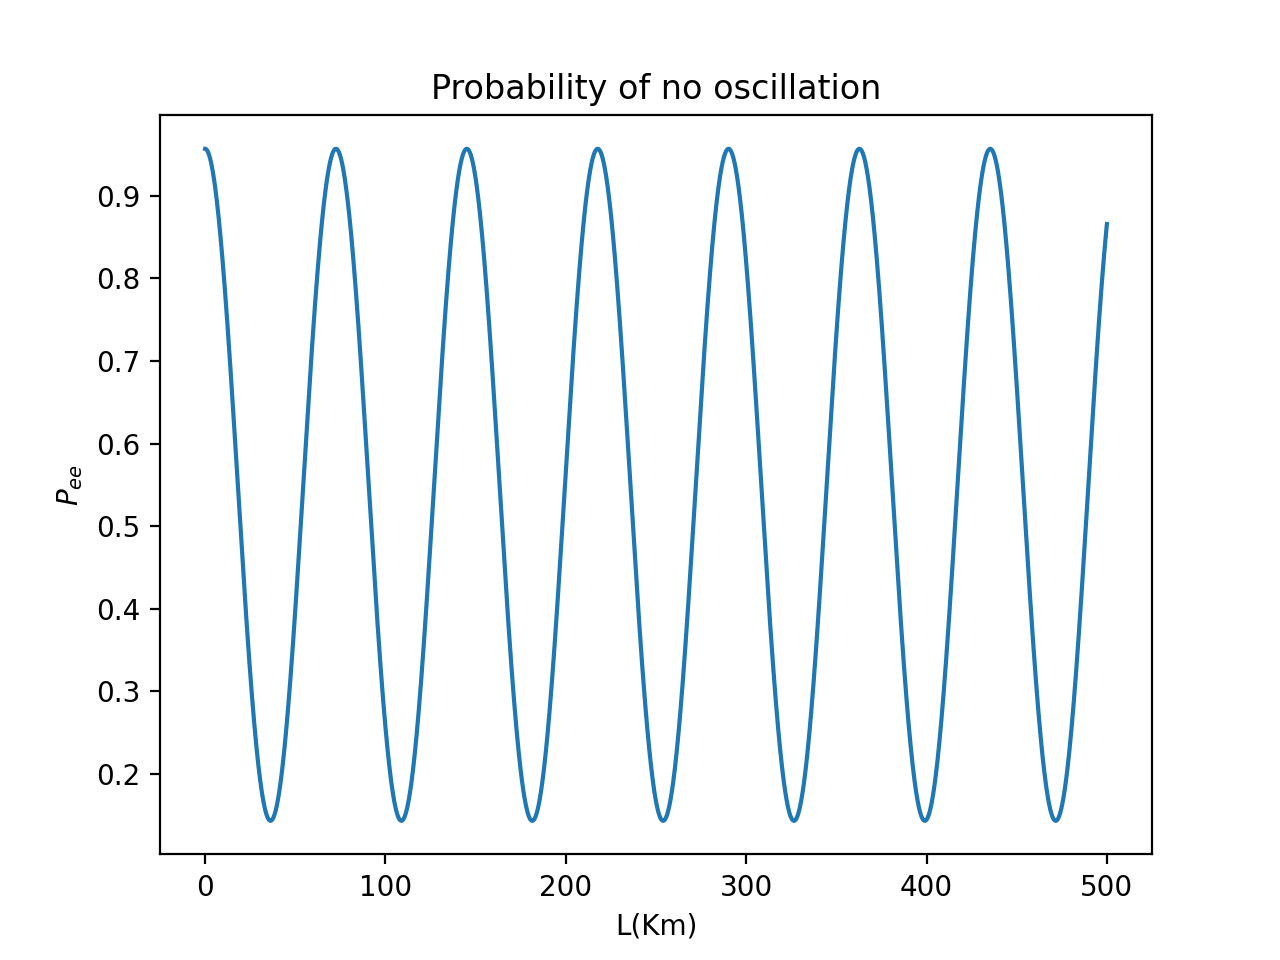
\includegraphics[width=0.7\linewidth]{no_oscillation.png}
	\caption{}
	\label{nooscillation}
\end{figure}\\
Filling in the values (again from the PDG) we get figure \ref{nooscillation}. The sine can be rewritten as $\sin(0.0433659\times L)$ thus, assuming that with oscillation length one period is meant, we have an oscillation length of $\frac{2\pi}{0.0433659} \approx 144.89$Km.\\
The earth's radius is $R_{\oplus} = 6.3781\times10^3$Km, if we assume the earth to be a sphere, then the average length a neutrino from anywhere within the earth will travel to a detector is the same as the length from the earth's core to the detector as everything perfectly cancels out. Thus if we fill in $R_{\oplus} = 6.3781\times10^3$Km into the equation we get $<P_{ee}> \approx 0.89$ or $89\%$ survival probability of the $\bar{\nu}_e$ state.
\subsection{Cross section for inverse $\beta$-decay}
The cross section for $\bar{\nu}_e p \rightarrow e^+ n$ is given by:
\begin{equation}
	\sigma = \frac{G_F^2}{\pi}(g_V^2+3g_A^2)(E_\nu-\Delta)\sqrt{(E_\nu-\Delta)^2-m_e^2}
\end{equation}
Filling in the values for an average geoneutrino energy of $E_\nu = 2.2$MeV we get $\sigma\approx9.62\times10^{-18}$mb$^2$ = $9.62\times10^{-45}$cm$^2$.
\subsection{number of detected geoneutrino events per year}
The total cross section is defined as:
\begin{equation}
	\sigma = \frac{\text{number of reactions per unit time}}{\text{beam particles per unit time}\times\text{scattering centres per unit area}}
\end{equation}
Assuming the detector to be a perfect cube then 1000 tons $= 1000\times10^3$kg (assuming metric tons) of water at 1000 kg/m$^3$ the bottom surface area (where the geoneutrinos are coming from) can be calculated as follows:
\begin{align}
	V_{\text{cube}} = L^3 &= \frac{1000\times10^3 \text{Kg}}{1000\text{Kg}}m^3 = 10^3 m^3\\
	\implies \text{area} &= L^2 = 10^2 m^2
\end{align}
As water has a molar mass of 18.01528 g/mol, 1 mol=6.02214076$\times10^{23}$ and we have 1000 tons of water, there are
\begin{equation}
	\frac{1000\times10^3}{18.01528\times10^{-3}}\times6.02214076\times10^{23} = 3.34\times10^{31} \text{ molecules}
\end{equation}
And thus $3.34\times10^{31}\times10 = 3.34\times10^{32}$ protons to interact with. This implies $\frac{3.34\times10^{32}}{10^2} = 3.34\times10^{30}$ scattering centres per square meter or $3.34\times10^{26}$ per cm$^2$. As we have previously calculated $f \approx 10^6$ geoneutrinos per unit area and time of which we'll detect a sixth ($\approx 1.66\times10^5$) as one in six has energy above the threshold and thus (surface in cm$^2\times$flux) $10^6\times1.66\times10^5 = 1.66\times10^{11}$ detectable geoneutrino's entering the volume every second. Using all this information we can calculate the number of reactions per unit time $\Omega$:
\begin{align}
	\Omega &= \sigma \times \text{beam particles per unit time} \times \text{scattering centres per unit area}\\
	 &= (9.62\times10^{-45}\text{cm}^2) \times (1.66\times10^{11} \text{s}^{-1}) \times (3.34\times10^{26}\text{ cm}^{-1})\\
	 &= 5.33\times10^{-7}\text{ s}^{-1}
\end{align}
This implies $\approx 5.33\times10^{-7} \times3600\times24\times365 \approx 17$ events per year.
\subsection{How can we measure geonetrinos when the sun produces a huge neutrino flux?}
The sun releases neutrinos, no antineutrinos, and it's only antineutrinos that can induce inverse $\beta$-decay. Terrestrial antineutrino observation relies on detecting both products of this inverse $\beta$ reaction to know for sure that we're not measuring solar neutrino interactions. The spatial and temporal coincidence of a prompt positron and delayed neutron capture distinctly identifies the interaction of an electron antineutrino.\cite{Geo-neutrinoObservation}. Another important source of background would be reactor neutrinos (from nuclear fission) as these are antineutrinos, a way to control this would be to build the detector as far away from a nuclear reactor as possible.
\bibliography{sources}
\bibliographystyle{plain}
\end{document}
